\documentclass[a4paper, 12pt]{article}

\usepackage[utf8]{inputenc}

\usepackage{graphicx}
\usepackage{caption}
\usepackage{parskip}

\usepackage{physics}
\usepackage{amsmath}

\usepackage{tikz}
\usepackage{tkz-graph}
\usepackage{tikzscale}
\usetikzlibrary{arrows}

\captionsetup{width=0.8 \linewidth}

\begin{document}

\title{\vspace{-6em}\textbf{Homework 5}\\ \Large Information Theory for Complex Systems \vspace{-3.2em} }
\author{} \date{March - 2023}

\maketitle

\section*{a)}
In order to show that $A = [0, 0.5], B = (0.5,1]$ is a generative partition we need to show that the subsets of $[0,1]$ corresponding to sequences of symbols increasing in length shrink over the interval and tend towards 0. Another way of wording this is that diam$(x_1 x_2 \dots x_m) \rightarrow 0$ as $m \rightarrow 0$.

\begin{figure}[ht!]
    \centering
    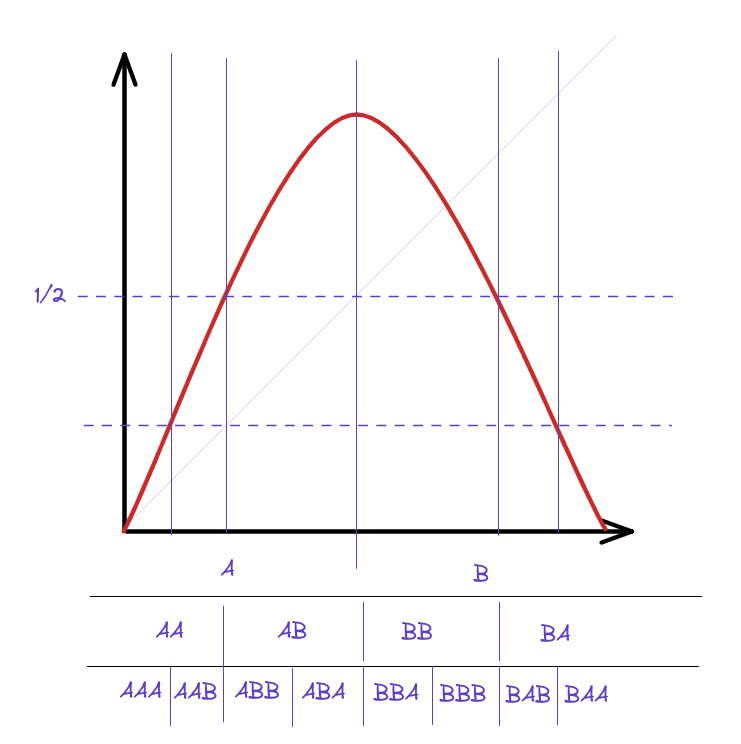
\includegraphics[width=0.5 \linewidth]{map.png}
\end{figure}

As can be seen in the figure, whenever we add another symbol to the sequence each interval is split into two subsets. As we can observe, there's always one subset with an $A$ added at the end and one with a $B$ at the end. The partition therefore enumerates all permutations of $A$ and $B$ uniquely. It's the same behaviour as in a binary tree (although each binary split doesn't split the interval in half). We get no disconnected sets, therefore all new splits shrink in size, equivalent with diam$(x_1 x_2 \dots x_m) \rightarrow 0$ as $m \rightarrow 0$.

\end{document}
